% answers.tex —— 2007 年·全国大纲卷Ⅱ·文科 · 参考答案与详细解析片段
% 由 tools/generate_projects.py 依来源总账自 2007/2007_数学真题_全国2文_试题.md + 2007/2007_数学真题_全国2文_解析正文.md + 2007/2007_数学真题_全国2文_答案要点.md 生成，勿手改（改源 MD 后重跑）


\begin{gktip}
固定源 PDF 为印刷页码 365–366 的两页题面，不附答案。以下解析均依据固定源独立复算；第 20 题图形在 LaTeX 工程中以 TikZ/PGFPlots 矢量源重绘。
\end{gktip}

\begin{answer}
\gksolhead{1}{}

\textbf{题目}：

$\cos330^\circ=$\mbox{（　　）}

（A）$\dfrac12$\quad（B）$-\dfrac12$\quad（C）$\dfrac{\sqrt3}{2}$\quad（D）$-\dfrac{\sqrt3}{2}$

\Needspace{4\baselineskip}
\textbf{解析}

\nopagebreak[4]
\[
\cos330^\circ=\cos30^\circ=\frac{\sqrt3}{2}
\]
。

\gkanswer{答案：C}

\end{answer}
\begin{answer}
\gksolhead{2}{}

\textbf{题目}：

设全集 $U=\{1,2,3,4\}$，$A=\{1,2\}$，$B=\{2,4\}$，则 $\complement_U(A\cup B)=$\mbox{（　　）}

（A）$\{2\}$\quad（B）$\{3\}$\quad（C）$\{1,2,4\}$\quad（D）$\{1,4\}$

\Needspace{4\baselineskip}
\textbf{解析}

$A\cup B=\{1,2,4\}$，在 $U$ 中的补集为 $\{3\}$。

\gkanswer{答案：B}

\end{answer}
\begin{answer}
\gksolhead{3}{}

\textbf{题目}：

函数 $f(x)=|\sin x|$ 的一个单调递增区间是\mbox{（　　）}

（A）$\left(-\dfrac\pi4,\dfrac\pi4\right)$\quad（B）$\left(\dfrac\pi4,\dfrac{3\pi}4\right)$\quad（C）$\left(\pi,\dfrac{3\pi}2\right)$\quad（D）$\left(\dfrac{3\pi}2,2\pi\right)$

\Needspace{4\baselineskip}
\textbf{解析}

在 $(\pi,3\pi/2)$ 内，$|\sin x|=-\sin x$ 且随 $x$ 递增，故为单调递增区间。

\gkanswer{答案：C}

\end{answer}
\begin{answer}
\gksolhead{4}{}

\textbf{题目}：

以下四个数中的最大者是\mbox{（　　）}

（A）$(\ln2)^2$\quad（B）$\ln(\ln2)$\quad（C）$\ln\sqrt2$\quad（D）$\ln2$

\Needspace{4\baselineskip}
\textbf{解析}

$(\ln2)^2<\ln2$，$\ln(\ln2)<0$，且 $\ln\sqrt2=\frac12\ln2$，故最大者为 $\ln2$。

\gkanswer{答案：D}

\end{answer}
\begin{answer}
\gksolhead{5}{}

\textbf{题目}：

不等式 $\dfrac{x-2}{x+3}>0$ 的解集是\mbox{（　　）}

（A）$(-3,2)$\quad（B）$(2,+\infty)$\quad（C）$(-\infty,-3)\cup(2,+\infty)$\quad（D）$(-\infty,-2)\cup(3,+\infty)$

\Needspace{4\baselineskip}
\textbf{解析}

临界点为 $-3,2$，作符号表得正区间为 $(-\infty,-3)\cup(2,+\infty)$。

\gkanswer{答案：C}

\end{answer}
\begin{answer}
\gksolhead{6}{}

\textbf{题目}：

在 $\triangle ABC$ 中，已知 $D$ 是 $AB$ 边上一点，若 $\overrightarrow{AD}=2\overrightarrow{DB}$，$\overrightarrow{CD}=\dfrac13\overrightarrow{CA}+\lambda\overrightarrow{CB}$，则 $\lambda=$\mbox{（　　）}

（A）$\dfrac23$\quad（B）$\dfrac13$\quad（C）$-\dfrac13$\quad（D）$-\dfrac23$

\Needspace{4\baselineskip}
\textbf{解析}

\Needspace{5\baselineskip}
由 $AD=2DB$，有 $D=(A+2B)/3$。所以

\nopagebreak[4]
\[
\overrightarrow{CD}=\frac13\overrightarrow{CA}+\frac23\overrightarrow{CB}
\]
，

得到 $\lambda=2/3$。

\gkanswer{答案：A}

\end{answer}
\begin{answer}
\gksolhead{7}{}

\textbf{题目}：

已知正三棱锥的侧棱长是底面边长的 $2$ 倍，则侧棱与底面所成角的余弦值等于\mbox{（　　）}

（A）$\dfrac{\sqrt3}{6}$\quad（B）$\dfrac{\sqrt3}{4}$\quad（C）$\dfrac{\sqrt2}{2}$\quad（D）$\dfrac{\sqrt3}{2}$

\Needspace{4\baselineskip}
\textbf{解析}

\Needspace{5\baselineskip}
底面中心到顶点的距离为 $a/\sqrt3$，侧棱为 $2a$，故侧棱与底面所成角 $\theta$ 的余弦为

\nopagebreak[4]
\[
\cos\theta=\frac{a/\sqrt3}{2a}=\frac{\sqrt3}{6}
\]
。

\gkanswer{答案：A}

\end{answer}
\begin{answer}
\gksolhead{8}{}

\textbf{题目}：

已知曲线 $y=\dfrac{x^2}{4}$ 的一条切线的斜率为 $\dfrac12$，则切点的横坐标为\mbox{（　　）}

（A）$1$\quad（B）$2$\quad（C）$3$\quad（D）$4$

\Needspace{4\baselineskip}
\textbf{解析}

曲线导数 $y'=x/2$，令 $x/2=1/2$ 得切点横坐标 $x=1$。

\gkanswer{答案：A}

\end{answer}
\begin{answer}
\gksolhead{9}{}

\textbf{题目}：

把函数 $y=e^x$ 的图象按向量 $\boldsymbol a=(2,0)$ 平移，得到 $y=f(x)$ 的图象，则 $f(x)=$\mbox{（　　）}

（A）$e^x+2$\quad（B）$e^x-2$\quad（C）$e^{x-2}$\quad（D）$e^{x+2}$

\Needspace{4\baselineskip}
\textbf{解析}

平移向量 $(2,0)$ 后，原图象上的点 $(u,e^u)$ 变为 $(u+2,e^u)$，故 $f(x)=e^{x-2}$。

\gkanswer{答案：C}

\end{answer}
\begin{answer}
\gksolhead{10}{}

\textbf{题目}：

$5$ 位同学报名参加两个课外活动小组，每位同学限报其中的一个小组，则不同的报名方法共有\mbox{（　　）}

（A）$10$ 种\quad（B）$20$ 种\quad（C）$25$ 种\quad（D）$32$ 种

\Needspace{4\baselineskip}
\textbf{解析}

\Needspace{5\baselineskip}
先选星期五的两人，再从余下三人中有序选星期六、星期日各一人：

\nopagebreak[4]
\[
\binom52\cdot3\cdot2=60
\]
。

\gkanswer{答案：B}

\end{answer}
\begin{answer}
\gksolhead{11}{}

\textbf{题目}：

已知椭圆的长轴长是短轴长的 $2$ 倍，则椭圆的离心率为\mbox{（　　）}

（A）$\dfrac13$\quad（B）$\dfrac{\sqrt3}{3}$\quad（C）$\dfrac12$\quad（D）$\dfrac{\sqrt3}{2}$

\Needspace{4\baselineskip}
\textbf{解析}

\Needspace{5\baselineskip}
长半轴为 $2b$，短半轴为 $b$，故

\nopagebreak[4]
\[
e=\sqrt{1-\frac{b^2}{(2b)^2}}=\frac{\sqrt3}{2}
\]
。

\gkanswer{答案：D}

\end{answer}
\begin{answer}
\gksolhead{12}{}

\textbf{题目}：

设 $F_1,F_2$ 分别是双曲线 $x^2-\dfrac{y^2}{9}=1$ 的左、右焦点，若点 $P$ 在双曲线上，且 $\overrightarrow{PF_1}\cdot\overrightarrow{PF_2}=0$，则 $|\overrightarrow{PF_1}+\overrightarrow{PF_2}|=$\mbox{（　　）}

（A）$\sqrt{10}$\quad（B）$2\sqrt{10}$\quad（C）$\sqrt5$\quad（D）$2\sqrt5$

\Needspace{4\baselineskip}
\textbf{解析}

$F_1F_2=2\sqrt{10}$。因 $\overrightarrow{PF_1}\perp\overrightarrow{PF_2}$，向量和的长度等于直角三角形斜边 $F_1F_2$，故为 $2\sqrt{10}$。

\gkanswer{答案：B}

\end{answer}
\begin{answer}
\gksolhead{13}{}

\textbf{题目}：

一个总体含有 $100$ 个个体，以简单随机抽样方式从总体中抽取一个容量为 $5$ 的样本，则指定的某个个体被抽到的概率为\gkblank{}。

\Needspace{4\baselineskip}
\textbf{解析}

指定个体被容量 $5$ 的简单随机样本抽中的概率为 $5/100=0.05$。

\gkanswer{答案：$0.05$}

\end{answer}
\begin{answer}
\gksolhead{14}{}

\textbf{题目}：

已知数列的通项 $a_n=-5n+2$，则其前 $n$ 项和为 $S_n=$\gkblank{}。

\Needspace{4\baselineskip}
\textbf{解析}

\nopagebreak[4]
\[
S_n=\sum_{k=1}^n(-5k+2)
=-\frac{5n(n+1)}2+2n
=-\frac{n(5n+1)}2
\]
。

\gkanswer{答案：$-\dfrac{n(5n+1)}2$}

\end{answer}
\begin{answer}
\gksolhead{15}{}

\textbf{题目}：

一个正四棱柱的各个顶点在一个直径为 $2\mathrm{cm}$ 的球面上。如果正四棱柱的底面边长为 $1\mathrm{cm}$，那么该棱柱的表面积为\gkblank{} $\mathrm{cm}^2$。

\Needspace{4\baselineskip}
\textbf{解析}

\Needspace{5\baselineskip}
球半径为 $1$，底面对角线平方为 $2$，故棱柱高满足 $h^2+2=4$，即 $h=\sqrt2$。表面积为

\nopagebreak[4]
\[
2+4\sqrt2
\]
。

\gkanswer{答案：$2+4\sqrt2$}

\end{answer}
\begin{answer}
\gksolhead{16}{}

\textbf{题目}：

$(1+2x^2)\left(x+\dfrac1x\right)^8$ 的展开式中常数项为\gkblank{}。（用数字作答）

\Needspace{4\baselineskip}
\textbf{解析}

$(x+x^{-1})^8$ 的常数项为 $\binom84=70$，$2x^2(x+x^{-1})^8$ 的常数项来自 $x^{-2}$ 项，为 $2\binom85=112$，总和为 $182$。

\gkanswer{答案：$182$}

\end{answer}
\begin{answer}
\gksolhead{17}{}

\textbf{题目}：

设等比数列 $\{a_n\}$ 的公比 $q<1$，前 $n$ 项和为 $S_n$。已知 $a_3=2,S_4=5S_2$，求 $\{a_n\}$ 的通项公式。

\Needspace{4\baselineskip}
\textbf{解析}

\Needspace{5\baselineskip}
设公比为 $q$，由 $a_3=2$ 和 $S_4=5S_2$ 得

\nopagebreak[4]
\[
1+q+q^2+q^3=5(1+q)
\Longrightarrow(q+1)(q-2)(q+2)=0
\]
。

\Needspace{5\baselineskip}
结合 $q<1$，得 $q=-1$ 或 $q=-2$，分别得到

\nopagebreak[4]
\[
a_n=2(-1)^{n-1}
\quad\text{\text{或}}\quad
a_n=\frac12(-2)^{n-1}
\]
。

\gkanswer{答案：$a_n=2(-1)^{n-1}$ 或 $a_n=\dfrac12(-2)^{n-1}$。}

\end{answer}
\begin{answer}
\gksolhead{18}{}

\textbf{题目}：

在 $\triangle ABC$ 中，已知内角 $A=\dfrac\pi3$，边 $BC=2\sqrt3$，设内角 $B=x$，周长为 $y$。

（1） 求函数 $y=f(x)$ 的解析式和定义域；

（2） 求 $y$ 的最大值。

\Needspace{4\baselineskip}
\textbf{解析}

\gksubpart{(1)}

\Needspace{5\baselineskip}
由正弦定理，$BC=2\sqrt3$ 对应 $A=\pi/3$，故外接圆半径为 $2$。于是

\nopagebreak[4]
\[
y=2\sqrt3+4\sin x+4\sin\left(\frac{2\pi}3-x\right)
=2\sqrt3+6\sin x+2\sqrt3\cos x
\]
，

定义域为 $0<x<2\pi/3$。

\gksubpart{(2)}

$6\sin x+2\sqrt3\cos x$ 的最大值为 $4\sqrt3$，在 $x=\pi/3$ 处取得，因此 $y_{\max}=6\sqrt3$。

\gkanswer{答案（1）：$y=2\sqrt3+6\sin x+2\sqrt3\cos x$，$0<x<\dfrac{2\pi}3$。}

\gkanswer{答案（2）：最大值为 $6\sqrt3$。}

\end{answer}
\begin{answer}
\gksolhead{19}{}

\textbf{题目}：

从某批产品中，有放回地抽取产品二次，每次随机抽取 $1$ 件，假设事件 $A$：“取出的 $2$ 件产品中至多有 $1$ 件是二等品”的概率 $P(A)=0.96$。

（1） 求从该批产品中任取 $1$ 件是二等品的概率 $p$；

（2） 若该批产品共有 $100$ 件，从中任意抽取 $2$ 件，求事件 $B$：“取出的 $2$ 件产品中至少有一件是二等品”的概率 $P(B)$。

\Needspace{4\baselineskip}
\textbf{解析}

\gksubpart{(1)}

由有放回抽取，$P(A)=1-p^2=0.96$，故 $p=1/5$。

\gksubpart{(2)}

\Needspace{5\baselineskip}
无放回抽取两件，二等品数为 $20$，一等品数为 $80$。至少一件二等品的概率为

\nopagebreak[4]
\[
1-\frac{\binom{80}{2}}{\binom{100}{2}}
=\frac{179}{495}
\]
。

\gkanswer{答案（1）：$p=\dfrac15$。}

\gkanswer{答案（2）：$P(B)=\dfrac{179}{495}$。}

\end{answer}
\begin{answer}
\gksolhead{20}{}

\textbf{题目}：

如图，在四棱锥 $S-ABCD$ 中，底面 $ABCD$ 为正方形，侧棱 $SD\perp$ 底面 $ABCD$，$E\text{、}F$ 分别是 $AB\text{、}SC$ 的中点。
\nopagebreak[4]
\begin{center}% 2007 年全国大纲卷Ⅱ文科第 20 题：正方形底面四棱锥
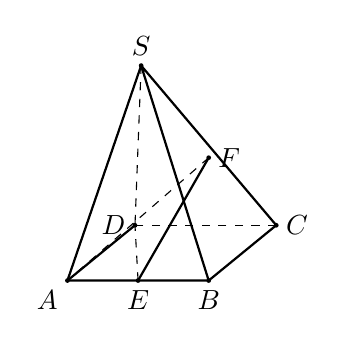
\begin{tikzpicture}[>=stealth,scale=0.78]
  \coordinate (A) at (0,0); \coordinate (B) at (2.3,0);
  \coordinate (C) at (3.4,0.9); \coordinate (D) at (1.1,0.9);
  \coordinate (S) at (1.2,3.5); \coordinate (E) at (1.15,0);
  \coordinate (F) at (2.3,2.0);
  \draw[thick] (A)--(B)--(C); \draw[dashed] (C)--(D); \draw[thick] (D)--(A);
  \draw[thick] (S)--(A) (S)--(B) (S)--(C);
  \draw[dashed] (S)--(D);
  \draw[thick] (E)--(F);
  \draw[dashed] (E)--(D) (F)--(A);
  \fill (S) circle (1.1pt) node[above] {$S$};
  \fill (A) circle (1.1pt) node[below left] {$A$};
  \fill (B) circle (1.1pt) node[below] {$B$};
  \fill (C) circle (1.1pt) node[right] {$C$};
  \fill (D) circle (1.1pt) node[left] {$D$};
  \fill (E) circle (1.1pt) node[below] {$E$};
  \fill (F) circle (1.1pt) node[right] {$F$};
\end{tikzpicture}
\end{center}
\nopagebreak[4]
（1） 求证：$EF\parallel$ 平面 $SAD$；

（2） 设 $SD=2CD$，求二面角 $A-EF-D$ 的大小。

\Needspace{4\baselineskip}
\textbf{解析}

\gksubpart{(1)}

取正方形底面边长为 $1$，设 $SD=h$，以底面建立坐标，则 $E$ 为 $AB$ 中点、$F$ 为 $SC$ 中点。直接计算可得 $\overrightarrow{EF}$ 为平面 $SAD$ 内的方向向量，故 $EF\parallel$ 平面 $SAD$。

\gksubpart{(2)}

\Needspace{5\baselineskip}
由 $SD=2CD$ 得 $h=2$。取两平面的法向量，计算得二面角 $\theta$ 满足

\nopagebreak[4]
\[
\cos\theta=\frac5{\sqrt{105}}
\]
。

\gkanswer{答案（1）：见解析版}

\gkanswer{答案（2）：二面角 $A-EF-D$ 满足 $\cos\theta=\dfrac5{\sqrt{105}}$。}

\end{answer}
\begin{answer}
\gksolhead{21}{}

\textbf{题目}：

在直角坐标系 $xOy$ 中，以 $O$ 为圆心的圆与直线 $x-3y=4$ 相切。

（1） 求圆 $O$ 的方程；

（2） 圆 $O$ 与 $x$ 轴相交于 $A,B$ 两点，圆内的动点 $P$ 使 $|PA|,|PO|,|PB|$ 成等比数列，求 $\overrightarrow{PA}\cdot\overrightarrow{PB}$ 的取值范围。

\Needspace{4\baselineskip}
\textbf{解析}

\gksubpart{(1)}

\Needspace{5\baselineskip}
圆心到直线距离为 $4/\sqrt{10}$，所以圆方程为

\nopagebreak[4]
\[
x^2+y^2=\frac85
\]
。

\gksubpart{(2)}

\Needspace{5\baselineskip}
令圆与 $x$ 轴交点为 $(\pm r,0)$，其中 $r^2=8/5$。等比条件平方后化简为

\nopagebreak[4]
\[
x^2-y^2=\frac45
\]
。

\Needspace{5\baselineskip}
结合圆内条件 $x^2+y^2<8/5$，有 $y^2<2/5$。而

\nopagebreak[4]
\[
\overrightarrow{PA}\cdot\overrightarrow{PB}=x^2+y^2-r^2=2y^2-\frac45
\]
，

故取值范围为 $\left(-\frac45,\frac45\right)$。

\gkanswer{答案（1）：圆为 $x^2+y^2=\dfrac85$。}

\gkanswer{答案（2）：$\overrightarrow{PA}\cdot\overrightarrow{PB}\in\left(-\dfrac45,\dfrac45\right)$。}

\end{answer}
\begin{answer}
\gksolhead{22}{}

\textbf{题目}：

已知函数 $f(x)=\dfrac13 ax^3-bx^2+(2-b)x+1$ 在 $x=x_1$ 处取得极大值，在 $x=x_2$ 处取得极小值，且 $0<x_1<1<x_2<2$。

（1） 证明 $a>0$；

（2） 若 $z=a+2b$，求 $z$ 的取值范围。

\Needspace{4\baselineskip}
\textbf{解析}

\gksubpart{(1)}

\Needspace{5\baselineskip}
令 $s=x_1+x_2,p=x_1x_2$。导数的两个根为 $x_1,x_2$，故

\nopagebreak[4]
\[
b=\frac{as}{2},\qquad 2-b=ap
\]
。

由于 $a>0$，取 $x_1\in(0,1),x_2\in(1,2)$。

\gksubpart{(2)}

\Needspace{5\baselineskip}
由上式

\nopagebreak[4]
\[
z=a+2b=\frac{4(1+x_1+x_2)}{2x_1x_2+x_1+x_2}
\]
。

\Needspace{5\baselineskip}
该式分别关于 $x_1,x_2$ 严格递减，边界极限给出

\nopagebreak[4]
\[
\frac{16}{7}<z<8
\]
。

\gkanswer{答案（1）：$a>0$。}

\gkanswer{答案（2）：$z\in\left(\dfrac{16}{7},8\right)$。}

\end{answer}